\documentclass[aspectratio=169, 11pt]{beamer}

% ====== Theme ======
\usetheme{Madrid}
\definecolor{CityUBlue}{RGB}{0, 51, 102}
\definecolor{CityULightBlue}{RGB}{0, 102, 179}
\definecolor{CityUGold}{RGB}{198, 163, 0}
\usecolortheme[named=CityUBlue]{structure}
\setbeamercolor{title}{fg=white, bg=CityUBlue}
\setbeamercolor{frametitle}{fg=white, bg=CityUBlue}
\setbeamercolor{block title}{bg=CityUBlue, fg=white}
\setbeamercolor{block body}{bg=CityUBlue!10, fg=black}
\setbeamercolor{item}{fg=CityUBlue}
\setbeamercolor{subitem}{fg=CityULightBlue}

% ====== Packages ======
\usepackage[T1]{fontenc}
\usepackage{lmodern}
\usepackage{booktabs}
\usepackage{graphicx}
\usepackage{hyperref}
\usepackage{amsmath, amssymb}
\usepackage{tikz}
\usepackage{appendixnumberbeamer}

% ====== Settings ======
\setbeamertemplate{navigation symbols}{}
\graphicspath{{figures/}{../../Figures used in slides/}}

% ====== Metadata ======
\title[EF8083 Lecture 2]{PhD Lecture in Behavioral Asset Pricing:\\ Limits to Arbitrage}
\author[F.\ W.\ Li]{Frank Weikai Li}
\institute[CityU]{Associate Professor of Finance\\City University of Hong Kong}
\date{}

% ==============================================================================
\begin{document}
% ==============================================================================

% --- Slide 1: Title ---
\begin{frame}[plain]
\titlepage
\end{frame}

% --- Slide 2: Overview ---
\section{Overview}

\begin{frame}{Overview}
\begin{itemize}
\item Behavioral finance applications to asset pricing posit that irrational investors affect prices
\item There is a classic critique of this idea
  \begin{itemize}
  \item The ``arbitrage critique''
  \end{itemize}
\item According to this critique, irrational investors cannot affect prices for any significant amount of time
  \begin{itemize}
  \item As soon as irrational investors move prices, this creates an attractive opportunity for rational investors
  \item The rational investors trade against the mispricing, quickly eliminating it (``arbitrage'')
  \end{itemize}
\item A major achievement of behavioural finance is to successfully push back against the arbitrage critique
  \begin{itemize}
  \item i.e.\ to show that there are ``limits to arbitrage''
  \end{itemize}
\end{itemize}
\end{frame}

% --- Slide 3: Overview, ctd. ---
\begin{frame}{Overview, ctd.}
\begin{itemize}
\item \textbf{Terminology:}
  \begin{itemize}
  \item The ``fundamental value'' of an asset is its price in an economy with rational investors and no frictions
    \begin{itemize}
    \item The price that properly reflects all available public information
    \item The efficient market price
    \end{itemize}
  \item In an economy with frictions, or where agents are not fully rational, an asset's price can depart from fundamental value
    \begin{itemize}
    \item This is a ``mispricing''
    \item Or an ``inefficiency''
    \end{itemize}
  \item Rational investors are sometimes referred to as ``arbitrageurs''
  \item Less than fully rational investors are sometimes referred to as ``noise traders''
  \end{itemize}
\end{itemize}
\end{frame}

% --- Slide 4: Overview, ctd. ---
\begin{frame}{Overview, ctd.}
\begin{itemize}
\item \textbf{Arbitrage}
  \begin{itemize}
  \item An investment strategy that guarantees a positive payoff in some state, with no possibility of a negative payoff, no net investment, and at arbitrary scale
  \end{itemize}
\item $\Rightarrow$ Money Machine
\item Arbitrage opportunities are inconsistent with common notions of equilibrium
  \begin{itemize}
  \item If arbitrage opportunities are there, then someone will act, and prices will change, so not a stable situation
  \end{itemize}
\item \textbf{Law of one price}
  \begin{itemize}
  \item Two assets with the same payoff in every state must have the same price
  \item Key to law of one price is perfect substitutes (exact same payoffs)
  \item Underlies much of the design of derivatives
  \end{itemize}
\end{itemize}
\end{frame}

% --- Slide 5: Limits to arbitrage: Theory ---
\section{Limits to Arbitrage: Theory}

\begin{frame}{Limits to Arbitrage: Theory}
\begin{itemize}
\item What is the response to the arbitrage critique?
  \begin{itemize}
  \item The arbitrage critique says that it will be easy for rational investors to correct a mispricing
  \item In reality, however, it is not easy
    \begin{itemize}
    \item There are risks and costs that limit arbitrageurs' ability to correct a mispricing
    \item This allows irrational investors to affect prices significantly and for a long time
    \end{itemize}
  \item Specific limits to arbitrage:
    \begin{itemize}
    \item \textbf{Risks:} fundamental risk, noise trader risk, horizon risk, model risk
    \item \textbf{Costs:} trading costs, shorting costs, identification costs
    \end{itemize}
  \end{itemize}
\end{itemize}
\end{frame}

% --- Slide 6: Fundamental risk ---
\begin{frame}{Limits to Arbitrage: Theory, ctd.}
\begin{itemize}
\item \textbf{Fundamental risk}
  \begin{itemize}
  \item The risk that there will be adverse news about the fundamental value of the mispriced asset
  \item Usually a problem because perfect substitutes are not available for what you really want to trade on
    \begin{itemize}
    \item E.g., You think Ford is underpriced, but your best hedge against unexpected changes is GM
    \end{itemize}
  \end{itemize}
\end{itemize}
\end{frame}

% --- Slide 7: Noise trader risk ---
\begin{frame}{Limits to Arbitrage: Theory, ctd.}
\begin{itemize}
\item \textbf{Noise trader risk} (De Long et al., 1990; Shleifer and Vishny, 1997)
  \begin{itemize}
  \item The risk that, as a result of the mispricing worsening in the short run, the arbitrageur is forced to close out his trade prematurely at a loss
  \item This risk arises because real-world arbitrageurs typically manage other people's money and because they use leverage
  \end{itemize}
\item \textbf{An example:}
  \begin{itemize}
  \item Arbitrageurs engage in arbitrage in reaction to a stock mispricing
  \item Mispricing persists for an extended period
  \item Clients deem the arbitrageur incompetent and demand fund withdrawal
  \item To deliver cash, manager must unwind the position at a loss
  \item This threat causes managers to be less prone to take advantage of these opportunities, exacerbating the problem of pricing inefficiency
  \end{itemize}
\end{itemize}
\end{frame}

% --- Slide 8: Leverage and short selling ---
\begin{frame}{Limits to Arbitrage: Theory, ctd.}
\begin{itemize}
\item Hedge funds' use of leverage and short selling compound the problem
  \begin{itemize}
  \item If a fund borrows money to buy an undervalued asset and the mispricing then worsens
  \item The lender, seeing the value of his collateral decline, may call the loan
  \item This forces the fund to close out its trade at a loss
  \item Similarly, if the fund shorts an overvalued asset and the asset then goes up in price
  \item The lender will demand additional margin
  \item If the fund cannot meet this demand, the short position will be closed out at a loss
  \item A fund manager who foresees these potential outcomes will trade less aggressively ex-ante against the mispricing
  \end{itemize}
\end{itemize}
\end{frame}

% --- Slide 9: Arbitrage In Reality ---
\section{Arbitrage In Reality}

\begin{frame}[shrink=5]{Arbitrage In Reality}
\vfill
\centering
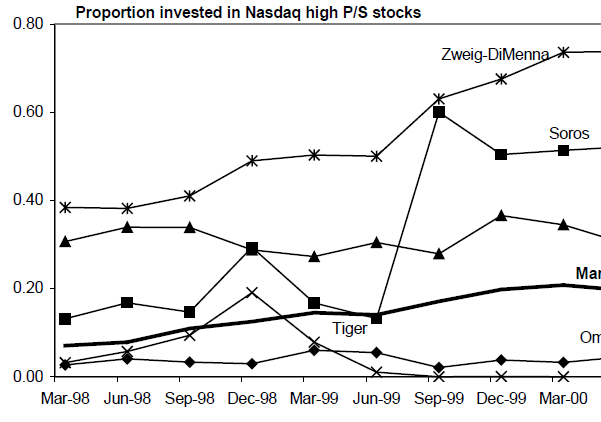
\includegraphics[width=0.65\textwidth]{figures/slide09_pic1.png}
\vfill
\end{frame}

% --- Slide 10: Arbitrage In Reality, ctd. ---
\begin{frame}[shrink=5]{Arbitrage In Reality, ctd.}
\vfill
\centering
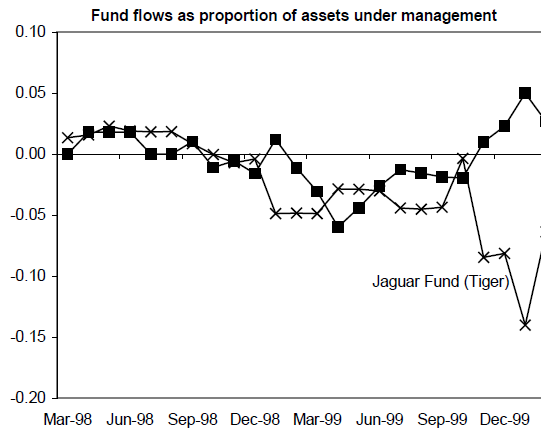
\includegraphics[width=0.75\textwidth]{figures/slide10_pic1.png}
\vfill
\end{frame}

% --- Slide 11: Trading costs ---
\begin{frame}{Limits to Arbitrage: Theory, ctd.}
\begin{itemize}
\item \textbf{Trading costs}
  \begin{itemize}
  \item Brokerage commissions
  \item Bid/Ask Spreads
  \item Price Impact
  \end{itemize}
\item \textbf{Shorting cost}
  \begin{itemize}
  \item Short selling involves borrowing shares from a lender, and need to pay lending fees
  \item The lending fees could be very high for certain stocks in certain periods
  \item Short selling are occasionally banned by regulators
  \item Some countries do not allow short selling at all
  \end{itemize}
\item \textbf{Information processing cost}
  \begin{itemize}
  \item Acquiring and processing financial statement data
  \end{itemize}
\end{itemize}
\end{frame}

% --- Slide 12: Dynamic arbitrage critique ---
\begin{frame}{Limits to Arbitrage: Theory, ctd.}
\begin{itemize}
\item Thus far, we have examined the ``static'' version of the arbitrage critique
\item There is also a dynamic version, which says:
  \begin{itemize}
  \item Even if rational traders are unable to quickly correct a mispricing, assets will eventually become correctly priced
  \item By trading sub-optimally, irrational traders become poorer over time
  \item As a result, they eventually become irrelevant to the pricing of assets
  \end{itemize}
\item This idea has generated a sizeable literature on the ``survival of noise traders''
\item How compelling is the dynamic arbitrage critique?
  \begin{itemize}
  \item It may take a very long time for irrational traders to exit market
  \item New generation of irrational investors enter the market
  \end{itemize}
\end{itemize}
\end{frame}

% --- Slide 13: Evidence ---
\section{Limits to Arbitrage: Evidence}

\begin{frame}{Limits to Arbitrage: Evidence}
\begin{itemize}
\item There are good theoretical reasons why arbitrage may be limited
  \begin{itemize}
  \item But is there evidence that arbitrage is limited?
  \end{itemize}
\item Any example of a substantial, long-lived mispricing would be evidence of limits to arbitrage
  \begin{itemize}
  \item But such examples are not easy to document
  \end{itemize}
\item Still, there are some pricing patterns that are widely viewed as mispricings
  \begin{itemize}
  \item These constitute evidence of limits to arbitrage
  \item And highlight the role played by each type of frictions
  \end{itemize}
\item Specifically, we look at:
  \begin{itemize}
  \item Twin shares
  \item Equity carve-outs
  \item Index inclusions
  \item Anomalies
  \end{itemize}
\end{itemize}
\end{frame}

% --- Slide 14: Twin shares ---
\begin{frame}{Twin Shares}
\begin{columns}[T]
\begin{column}{0.50\textwidth}
\begin{itemize}
\item Twin shares are distinct shares that are claims to the same cash flows
\item In 1907, Royal Dutch and Shell merged their interests while remaining separate entities
  \begin{itemize}
  \item Royal Dutch has a claim to 60\% of the combined firm's cash flows
  \item Shell has a claim to 40\% of the combined firm's cash flows
  \end{itemize}
\item In an economy with rational investors and no frictions, the ratio of market values of equity should be:
\[
\text{Price}_{RD} = 1.5 \times \text{Price}_{S}
\]
\end{itemize}
\end{column}
\begin{column}{0.48\textwidth}
\centering
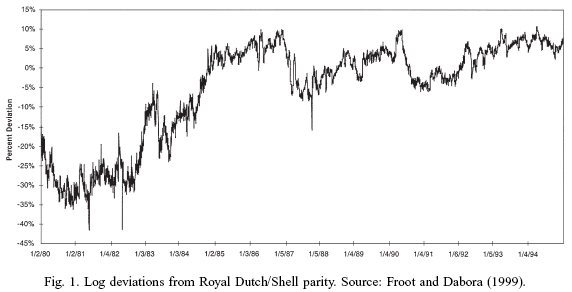
\includegraphics[width=\textwidth]{figures/slide14_pic1.png}\\[0.2em]
\footnotesize This is a long-lived mispricing, and is therefore also evidence that it is hard to correct a mispricing
\end{column}
\end{columns}
\end{frame}

% --- Slide 15: Twin shares, ctd. ---
\begin{frame}{Twin Shares, ctd.}
\begin{columns}[T]
\begin{column}{0.50\textwidth}
\begin{itemize}
\item \textbf{Example: AH Premium}
  \begin{itemize}
  \item Dozens of Chinese companies' stocks are listed in both China's domestic stock market (A shares) and Hong Kong stock market (H shares)
  \item A shares are usually traded at premium over H shares of the same company
  \end{itemize}
\end{itemize}
\end{column}
\begin{column}{0.48\textwidth}
\centering
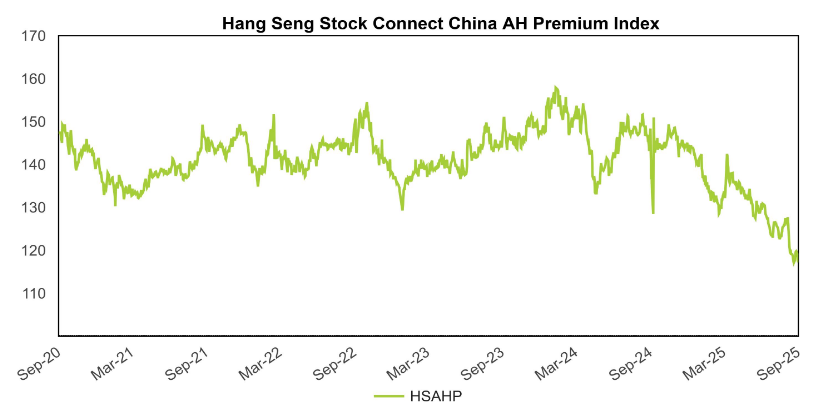
\includegraphics[width=\textwidth]{figures/slide15_pic1.png}
\end{column}
\end{columns}
\end{frame}

% --- Slide 16: Equity carve-outs ---
\begin{frame}{Equity Carve-Outs}
\begin{itemize}
\item Mitchell, Pulvino, and Stafford (2002) study equity carve-outs between 1985 and 2000
  \begin{itemize}
  \item Cases where a parent company conducts an IPO for shares in a subsidiary firm and retains 80\%+ ownership
  \end{itemize}
\item They find 70 cases where $MV_{Parent} < 0.8 \times MV_{Subsidiary}$
  \begin{itemize}
  \item Implies that parents' ``Stub'' assets are negative
  \end{itemize}
\item Why is this mispricing hard to correct?
  \begin{itemize}
  \item Fundamental risk (in 30\% of cases, there is adverse fundamental news)
  \item Noise trader risk
  \item Shorting costs
  \end{itemize}
\end{itemize}
\end{frame}

% --- Slide 17: Palm/3Com ---
\begin{frame}{Equity Carve-Outs, ctd.}
\begin{itemize}
\item \textbf{Palm/3Com}
  \begin{itemize}
  \item 3Com sells 5\% of Palm in IPO, will spin off remainder in 9 months
  \item 1 Share of 3Com will own 1.5 Shares of Palm
  \item $P_{Palm} = \$95$
  \item $P_{3Com}$ should be $\geq \$142$
  \item $P_{3Com} = \$81$
  \item Value of 3Com excluding Palm $= -\$60$ !!
  \item Very few shares of Palm available to short
  \end{itemize}
\end{itemize}
\end{frame}

% --- Slide 18: Index inclusions ---
\begin{frame}{Index Inclusions}
\begin{itemize}
\item Stocks are regularly added to the S\&P 500 index to replace other stocks that have been removed due to merger or bankruptcy
\item \textbf{Facts:} both on the announcement and execution days, the included stocks jump significantly in price by 3.5\% on average, and the jump is not reversed
  \begin{itemize}
  \item Harris and Gurel (1986), Shleifer (1986)
  \end{itemize}
\item The price jump is widely viewed as a mispricing
  \begin{itemize}
  \item S\&P's goal is to create a representative index, not to send signals about the included stocks' investment value
  \item As such, the effect is evidence that there are limits to arbitrage
  \end{itemize}
\item To correct the mispricing, an arbitrageur would short the included stocks and buy substitute stocks
  \begin{itemize}
  \item What are the limits to arbitrage in this case?
  \end{itemize}
\end{itemize}
\end{frame}

% --- Slide 19: Index inclusions, ctd. ---
\begin{frame}{Index Inclusions, ctd.}
\begin{itemize}
\item Wurgler and Zhuravskaya (2002) show that included stocks with worse substitutes (higher idiosyncratic risk) jump up more upon inclusion
\end{itemize}
\vfill
\centering
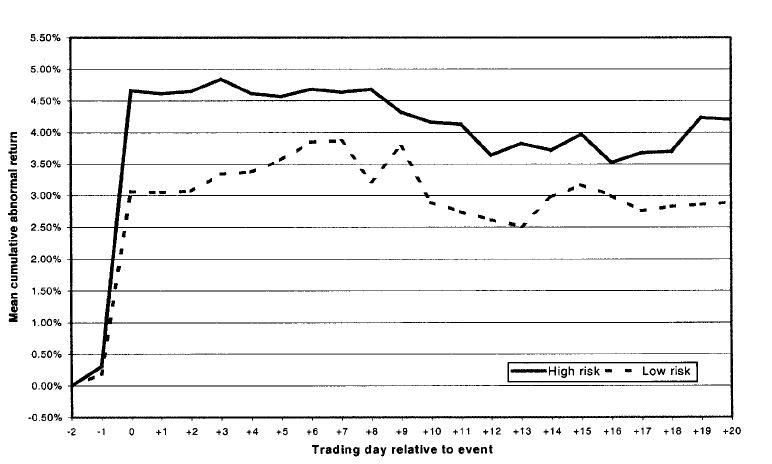
\includegraphics[width=0.60\textwidth]{figures/slide19_pic1.jpg}
\end{frame}

% --- Slide 20: Disappearing index effect ---
\begin{frame}{The Disappearing Index Effect}
\begin{itemize}
\item The abnormal return associated with a stock being added to the S\&P 500 has fallen from an average of 7.4\% in the 1990s to less than 1\% over the past decade (Greenwood and Sammon JF 2025)
\item This has occurred despite a significant increase in the share of stock market assets linked to the index
\item The main reason is professional active investors provide liquidity to accommodate the demand of passive indexers
\item Although index trackers now buy about 7--8\% upon index addition, total institutional ownership barely moves around index changes
\end{itemize}
\end{frame}

% --- Slide 21: Anomalies ---
\begin{frame}[shrink=5]{Anomalies}
\begin{itemize}
\item If anomalies are the result of mispricing, they should be more pronounced among stocks with more severe limits to arbitrage
  \begin{itemize}
  \item Using institutional ownership as proxy for short-sale constraints, Nagel (2005) finds the short-leg of anomalies is stronger among stocks with lower institutional ownership
  \item Using idiosyncratic volatility as proxy for arbitrage risk, Stambaugh, Yu and Yuan (2015) find mispricing is amplified among stocks with highest idiosyncratic volatility
  \end{itemize}
\end{itemize}
\vfill
\centering
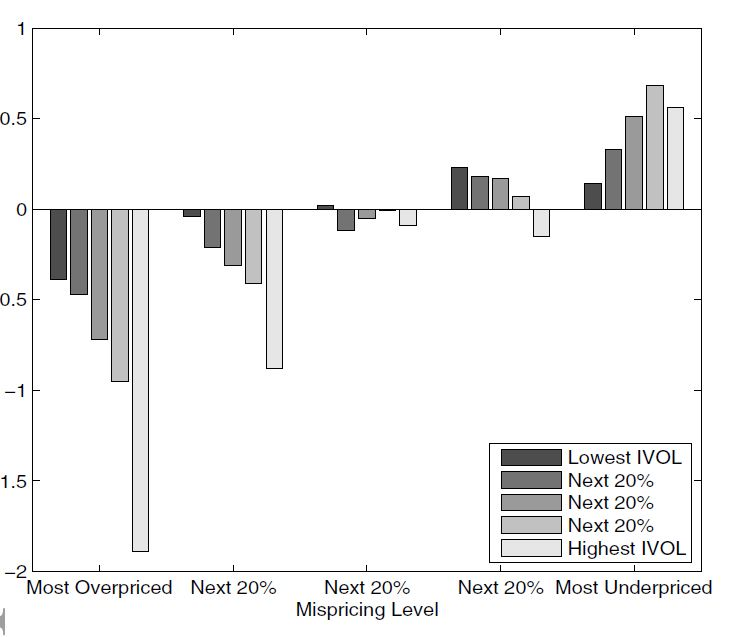
\includegraphics[width=0.55\textwidth]{figures/slide21_pic1.jpg}\\[0.2em]
\footnotesize Stambaugh, Yu and Yuan (2015)
\end{frame}

% --- Slide 22: Causal effects ---
\begin{frame}{The Causal Effects of Limits to Arbitrage}
\begin{itemize}
\item Chu, Hirshleifer and Ma (2020) show the causal effects of limits to arbitrage on asset pricing anomalies
\item They use Regulation SHO as a quasi-experiment:
  \begin{itemize}
  \item SEC removes short sale restrictions on a randomly selected group of stocks (pilot stocks) within Russell 3000 index
  \item The pilot program period is from May 2, 2005 to August 6, 2007
  \end{itemize}
\item Research design is standard differences-in-differences test:
  \begin{itemize}
  \item Construct anomaly long-short portfolios for pilot stocks and non-pilot stocks separately
  \item Compare the return spread of the long-short portfolios for pilot firms relative to non-pilot firms, before and during the pilot period
  \end{itemize}
\item Their main findings are:
  \begin{itemize}
  \item Anomalies become weaker for pilot stocks relative to non-pilot stocks during the pilot period
  \item The effect comes mostly from the short leg portfolio
  \end{itemize}
\end{itemize}
\end{frame}

% --- Slide 23: Causal effects, ctd. ---
\begin{frame}{The Causal Effects of Limits to Arbitrage, ctd.}
\vfill
\centering

\includegraphics[width=0.75\textwidth]{figures/slide23_pic1.jpg}\\[0.2em]
\footnotesize Chu, Hirshleifer, and Ma (2020)
\vfill
\end{frame}

% --- Slide 24: Information processing costs ---
\begin{frame}[shrink=5]{Information Processing Costs as Limit to Arbitrage}
\begin{itemize}
\item Bowles, Reed, Ringgenberg and Thornock (JF 2024)
\item Anomaly returns are concentrated in the first month after anomaly-relevant information is first released, and the returns decay quickly thereafter
\end{itemize}
\vfill
\centering
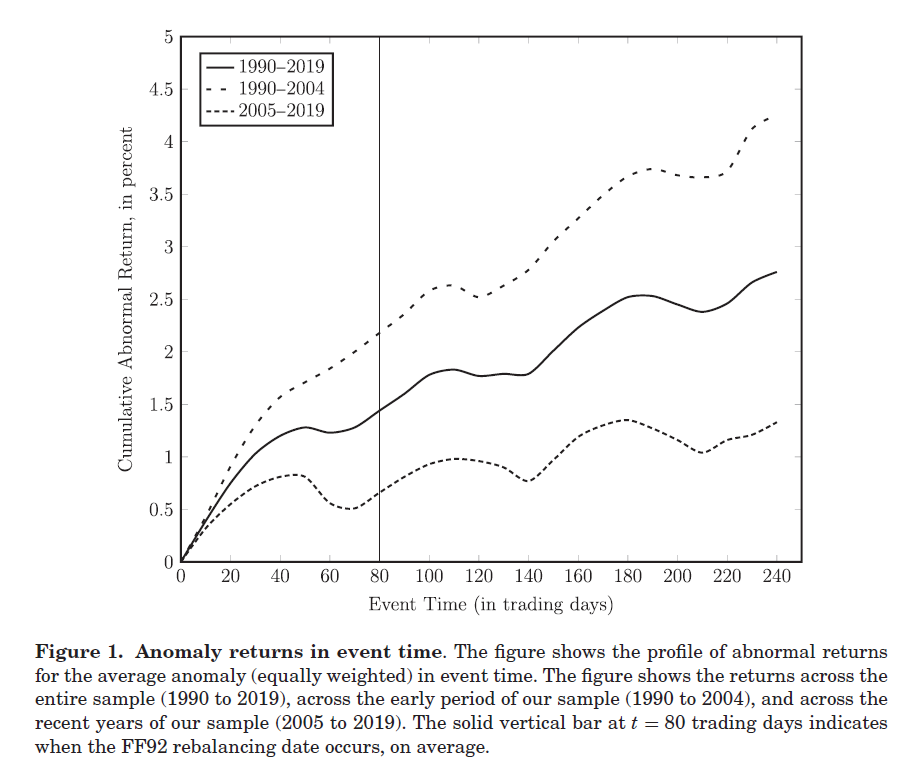
\includegraphics[width=0.75\textwidth]{figures/slide24_pic1.png}
\end{frame}

% --- Slide 25: Summary ---
\section{Summary}

\begin{frame}{Summary}
\begin{itemize}
\item The literature on limits to arbitrage has been influential
  \begin{itemize}
  \item There is now wide agreement among academics (and practitioners) that arbitrage is limited
  \item Albeit some disagreement as to how limited it is
  \end{itemize}
\item This success was one reason why behavioural finance ``took off'' in the 1990s
\item Still, we should not be complacent
  \begin{itemize}
  \item Whenever we argue that irrational investors' demand affect prices, we should ask if arbitrage is truly limited
  \end{itemize}
\end{itemize}
\end{frame}

\end{document}
